\section{Comparison with \\AMC, pATL$^*$ and $\mu$-pCTL}

The logics we compared in this section are defined over concurrent game structures (CGSs). % and Markov decision processes (MDPs).
Therefore, we first recall the definition of CGSs. 

\subsection{Concurrent Game Structures}

A pCGS $\calM=(\Ag,\Act, Q, \delta,\lambda,q_0)$ is a \emph{concurrent game structure} (CGS),
if $\delta$ is defined as $Q\times \calD\times Q\rightarrow \{0,1\}$ such that for every $q\in Q$ and
$\dec\in\calD$, there exists exactly one state $q'\in Q$ such that $\delta(q,\dec,q')=1$. We will use $\delta(q,\dec)$ to denote the unique state $q'$ such that  $\delta(q,\dec,q')=1$.
Strategies used by agents in CGSs are also deterministic.
In this setting, given a coalition strategy $\upsilon_A\in V_A$ and a response strategy $\upsilon_{\nA}\in V_{\nA}$ of agents $A$,
for every state $q\in Q$, $\calP_q^{\upsilon_A,\upsilon_{\nA}}$ is a singleton set. We use $\rho_q^{\upsilon_A,\upsilon_{\nA}}$ to denote the path
in $\calP_q^{\upsilon_A,\upsilon_{\nA}}$.
 
A pCGS $\calM=(\Ag,\Act, Q, \delta,\lambda,q_0)$ is a \emph{Markov decision process} (MDP) if $\calM$ is a one-agent pCGS, i.e., $|\Ag|=1$.


\subsection{Alternating-time $\mu$-Calculus}
Alternating-time $\mu$-calculus (AMC) is a powerful alternating-time temporal logic that is strictly more expressive than ATL and ATL$^*$.
We show that \pamcs is strong enough to express AMC over CGSs.
AMC is an extension of $\mu$-calculus with coalition modalities \cite{AHK02}.

\begin{definition}\cite{AHK02} AMC formulae are given by the following grammar:
\[\phi::= p \mid \neg p \mid Z \mid \phi\wedge \phi \mid \phi\vee \phi \mid \opA{A}\opX \phi \mid  \opUA{A}\opX \phi \mid  \mu Z.\phi\mid \nu Z.\phi\]
where $p\in \AP$, $Z\in \calZ$, $A\subseteq  \Ag$.
\end{definition}


The semantics of AMC formulae are defined by the denotation function $\|\circ\|_\calM^\xi$ that maps an AMC formula to a set of states of a CGS $\calM$.
%Due to space restriction, its detailed definition is omitted here and we refer to, e.g., \cite{AHK02}.
Formally, given a CGS  $\calM=(\Ag,\Act, Q, \delta,\lambda,q_0)$, an AMC formula $\phi$ and a valuation $\xi:\calZ\rightarrow 2^Q$,
$\|\circ\|_\calM^\xi$ is inductively defined as follows:

\begin{itemize}
  \item $\semantics{p}_\calM^\xi=\lambda(p)$, $\semantics{\neg p}_\calM^\xi=Q\setminus \lambda(p)$, $\semantics{Z}_\calM^\xi=\xi(Z)$;
  \item $\semantics{\opA{A}\opX \psi}_\calM^\xi= \{ \ q\in Q\mid \exists \upsilon_A\in V_A, \ \forall \upsilon_{\nA}\in V_{\nA},  \delta(q,\dec)\in \semantics{\psi}_\calM^\xi \}$, where $\upsilon_A(i)(q,\dec(i))=1$ for every $i\in A$ and $\upsilon_{\nA}(j)(q,\dec(j))=1$ for every $j\in \nA$;
  \item $\semantics{\opUA{A}\opX \psi}_\calM^\xi= \{ \ q\in Q\mid \forall \upsilon_A\in V_A, \ \exists \upsilon_{\nA}\in V_{\nA}, \delta(q,\dec)\in \semantics{\psi}_\calM^\xi \}$, where $\upsilon_A(i)(q,\dec(i))=1$ for every $i\in A$ and $\upsilon_{\nA}(j)(q,\dec(j))=1$ for every $j\in \nA$;
  \item $\semantics{\mu Z. \phi}_\calM^\xi=\bigcap\{Q'\subseteq Q\mid \semantics{\phi}_\calM^{\xi[Z\mapsto Q']}\subseteq Q'\}$;
  \item	$\semantics{\nu Z. \phi}_\calM^\xi=\bigcup\{Q'\subseteq Q\mid \semantics{\phi}_\calM^{\xi[Z\mapsto Q']}\supseteq Q'\}$;
  \item $\semantics{\phi_1\wedge \phi_2}_\calM^\xi=\semantics{\phi_1}_\calM^\xi\cap\semantics{\phi_2}_\calM^\xi$;
 \item $\semantics{\phi_1\vee \phi_2}_\calM^\xi=\semantics{\phi_1}_\calM^\xi\cup\semantics{\phi_2}_\calM^\xi$.
\end{itemize}

Given an AMC formula $\phi$, let $enc(\phi)$ denote the formula obtained from $\phi$ by the following recursive transformation:
where $\circ\in\{\wedge,\vee\}$,
\[\begin{array}{cc}
  enc(p)=p &  enc(\phi_1\circ \phi_2)=enc(\phi_1)\circ enc(\phi_2) \\
  enc(\neg p)=\neg p & enc(\opA{A}\opX \phi) = \opA{A}^{>0}\opX enc(\phi) \\
  enc(Z)=Z & enc(\opUA{A}\opX \phi) = \opUA{A}^{>0}\opX enc(\phi)\\
  enc( \mu Z.\phi)= \mu Z.enc(\phi)   & enc( \nu Z.\phi)= \nu Z.enc(\phi)
\end{array}\]

\begin{theorem}
For every CGS $\calM$ and every AMC formula $\phi$, $\semantics{\phi}_\calM^\xi=\semantics{enc(\phi)}_\calM^\xi$.
\end{theorem}

It is known that AMC is more expressive than ATL and ATL$^*$ \cite{AHK02}.
It follows that \pamcs is strong enough to express all standard alternating-time temporal logics.


\subsection{Probabilistic Alternating-time Temporal Logic}
Probabilistic alternating-time temporal logic (pATL$^*$) is the first probabilistic extension of the alternating-time temporal logic ATL$^*$ \cite{CL07a,Sch10,HSZ12}.

\begin{definition}pATL$^*$ formulae are given by the following grammar: where $\Phi$ are state formulae, $\Psi$ are path formulae,
$$\begin{array}{cl}
  \Phi::= & p \mid \neg p  \mid \Phi\wedge \Phi \mid \Phi\vee \Phi \mid \opA{A}^{\sim c}\Psi \mid  \opUA{A}^{\sim c}\Psi \\
  \Psi::= & \Phi\mid \Psi\wedge \Psi \mid \Psi\vee \Psi \mid  \opX \Psi \mid \Psi \opU \Psi   \mid \opR\Psi
\end{array}$$
where $p\in \AP$, $Z\in \calZ$, $A\subseteq  \Ag$, $\sim\in\{\geq, >\}$ and $c\in[0,1]$.
\end{definition}

\begin{remark}
The original definition of pATL$^*$ in \cite{CL07a} allows $\sim$ to be $=$, which is dropped in the later works \cite{Sch10,HSZ12}.
\pamc  disallows $\sim$ to be $=$. Therefore, we drop $=$ in the definition of pATL$^*$. This is not a strict restriction, as we could also allow $\sim$ to be $=$ as well.
\end{remark}

The semantics of path formulae and state formulae of pATL$^*$ are given by the denotation function $\|\circ\|_\calM^\xi$ and $\|\circ\|_\calM^{\xi,\rho}$ which are inductively defined similar as \pamc,
in which
$\|\psi_1\opU\psi_2\|_\calM^{\xi,\rho}\equiv \|\mu_p Z.\psi_2\vee (\psi_1\wedge \opX Z)\|_\calM^{\xi,\rho}$ and
$\|\psi_1\opR\psi_2\|_\calM^{\xi,\rho}\equiv \|\nu_p Z.(\psi_1\wedge \psi_2)\vee (\psi_2\wedge \opX Z)\|_\calM^{\xi,\rho}$.


Given a pATL$^*$ formula $\phi$, let $enc(\phi)$ denote the formula obtained from $\phi$ by the following recursive transformation:
where $\circ\in\{\wedge,\vee\}$,

\begin{center}
\begin{tabular}{cc}
 $enc(p)=p$ & $enc(\phi_1\circ \phi_2)=enc(\phi_1)\circ enc(\phi_2)$  \\
  $enc(\neg p)=\neg p$ & $enc(\opA{A}^{\sim c}\opX \phi) = \opA{A}^{\sim c}\opX enc(\phi)$   \\
 $enc(\opX \phi)=\opX enc(\phi)$ & $enc(\opUA{A}^{\sim c}\opX \phi) = \opUA{A}^{\sim c}\opX enc(\phi)$  \\
   \multicolumn{2}{c}{$enc(\phi_1\opU\phi_2)=\mu_p Z.enc(\phi_2)\vee (enc(\phi_1)\wedge \opX Z)$}\\
   \multicolumn{2}{c}{$enc(\phi_1\opR\phi_2)=\nu_p Z.enc(\phi_1\wedge \phi_2)\vee (enc(\phi_2)\wedge \opX Z)$}\\
\end{tabular}
\end{center}


pATL is a subclass of pATL$^*$ in which path formulae are given by: $\Psi::=\opX \Phi \mid \Phi \opU \Phi   \mid \opR\Phi$, where
$\Phi$ are state formulae. Similar to the transformation from pATL$^*$ to \pamc,
pATL formulae can be encoded into \pamcc.


\begin{lemma}
Every pATL$^*$ (resp. pATL) state formula $\phi$,
we can construct a \pamc (resp. \pamcc) formula $enc(\phi)$ such that $\semantics{\phi}_\calM=\semantics{enc(\phi)}_\calM$ for all pCGSs $\calM$.
\end{lemma}


Similar to the relation between AMC and ATL$^*$, fixpoint operators cannot be expressed in pATL$^*$, we get that:

\begin{theorem}
\pamc is strictly more expressive than pATL$^*$, and \pamcc is strictly more expressive than pATL.
\end{theorem}





\subsection{$\mu$-pCTL}
$\mu$-pCTL was introduced by \cite{CKP15} for reasoning about probabilistic systems, like Markov chain and Markov decision processes.
$\mu$-pCTL is able to encode several well-known probabilistic such as pCTL and p$\mu$TL \cite{LSWZ15}.


\begin{definition}[$\mu$-pCTL]
The syntax of probabilistic $\mu$-pCTL is given by the following grammar, where
$\Phi$ are \emph{state formulae}, $\Psi$ are \emph{path formulae},
 \[\begin{array}{l}
\Phi::=p\mid  \ \neg p \mid  \ Z \ \mid \Phi \wedge \Phi  \ \mid  \ \Phi \vee \Phi \ \mid \  \mu Z. \Phi  \ \mid \ \nu Z. \Phi  \  \mid \ [\Psi]^{\sim c} \\
\Psi::= \opX \Phi \ \mid \  \Phi \opU \Phi \ \mid  \ \Phi \opR \Phi \\
 \end{array}\]
where $p\in\AP$, $Z\in \calZ$, $c\in[0,1]$ and $\sim\in\{\geq,>\}$.
\end{definition}

The semantics of $\mu$-pCTL formulae are defined over MDPs (note that the semantics are defined over Markov chains in \cite{CKP15}).
Given a MDP $\calM=(\Ag,\Act, Q, \delta,\lambda,q_0)$, a state formula $\phi$ and a valuation $\xi:Z\rightarrow 2^Q$,
the denotation function $\|\circ\|_\calM^\xi$ that maps each state formula to a set of states is inductively defined as same as \pamc.
The semantics of path formulae is defined similar to \pamcc.

Given a $\mu$-pCTL formula $\phi$, it is easy to transform $\phi$ into an equivalent \pamcc formula
$enc(\phi)$ using  $enc([\psi]^{\sim c}) = \opA{\Ag}^{\sim c} enc(\psi)$.


\begin{theorem}
For every MDP $\calM$ and every $\mu$-pCTL state formula $\phi$, $\semantics{\phi}_\calM^\xi=\semantics{enc(\phi)}_\calM^\xi$.
\end{theorem}



\section{Memorability and Determinacy}
In this section, we show that the memoryless property of \pamcc,  hence \pamcs as well.
However, in general, \pamc does not have memoryless property.
For determinacy, we show that there is no difference between randomized and deterministic
under memoryful setting for \pamc. However, allowing $\sim\in\{\geq,>,=\}$ or only considering memoryless strategies
will lose this determinacy property.


\subsection{Memoryless vs. Memoryful}
\begin{proposition}\label{prop:one-step}Given a principal formula $\phi=\opA{A}^{\sim c}\opX\psi$ (resp. $\phi=\opUA{A}^{\sim c}\opX\psi$), and the coalition strategy $\upsilon_A$ and the response strategy
$\upsilon_{\nA}$ of $A$, for every state $q\in Q$, we have the following property:
$\Prb_q^{\upsilon_A,\upsilon_{\nA}}(\{ \ \rho\in \calP_q^{\upsilon_A,\upsilon_{\nA}}\mid \rho_1\in\semantics{\psi}_\calM^\xi \ \}) = \sum\limits_{\dec \in\calD , q'\in \semantics{\psi}_\calM^\xi} \Prb^{\upsilon_A,\upsilon_{\nA}}(q,\dec)\cdot \delta(q,\dec,q').$

%$\Prb_q^{\upsilon_A,\upsilon_{\nA}}(\{\rho\in \calP_q^{\upsilon_A,\upsilon_{\nA}}\mid \semantics{\phi_1}_\calM^\xi\})=\bigcup_{q_1\in %\semantics{\phi}_\calM^\xi}\Prb_q^{\upsilon_A,\upsilon_{\nA}}(\Cycl^{\upsilon_A,\upsilon_{\nA}}(qq_1)) \cdot \sum_{\dec\in \calD} p_{\dec}^1\cdot p_{\dec}^2\cdot\delta(q,\dec,q_1)$,
%where $p_{\dec}^1=\prod_{j\in A} \upsilon_A(j)(q)(\dec(j))$ and $p_{\dec}^2=\prod_{j\in \nA} \upsilon_{\nA}(j)(q)(\dec(j))$.
\end{proposition}
\begin{proof}
The result immediately follows from the fact that
$\{ \ \rho\in \calP_q^{\upsilon_A,\upsilon_{\nA}}\mid \rho_1\in\semantics{\psi}_\calM^\xi \ \}=\bigcup_{q'\in \semantics{\psi}_\calM^\xi}\Cycl^{\upsilon_A,\upsilon_{\nA}}(qq')$.
\end{proof}




\begin{proposition}\label{prop-mc-pamc-memless}
Given a pCGS $\calM=(\Ag,\Act, Q, \delta,\lambda,q_0)$ and a closed \pamcc state formula $\phi$,
let $\semantics{\phi}_\calM^R$ and $\semantics{\phi}_\calM^r$ respectively denote the set of states
satisfying $\phi$ under memoryful and memoryless settings. Then,
$\semantics{\phi}_\calM^R=\semantics{\phi}_\calM^r$.
\end{proposition}
\begin{proof}
By applying induction on structure, it is sufficient to show the cases for $\phi=\opA{A}^{\sim c}\opX\psi$, $\phi=\opUA{A}^{\sim c}\opX\psi$,
$\phi=\opA{A}^{\sim c}\psi_1\opU\psi_2$, $\phi=\opUA{A}^{\sim c}\psi_1\opU\psi_2$, $\phi=\opA{A}^{\sim c}\psi_1\opR\psi_2$ and $\phi=\opUA{A}^{\sim c}\psi_1\opR\psi_2$.

Let us consider the case $\phi=\opA{A}^{\sim c}\opX\psi$.
Since $q\in \semantics{\opA{A}^{\sim c}\opX\psi}_\calM^\xi$ iff there exists $\upsilon_A\in V_A$ such that for every $\upsilon_{\nA}\in V_{\nA}$: $\Prb_q^{\upsilon_A,\upsilon_{\nA}}(\{\rho\in \calP_q^{\upsilon_A,\upsilon_{\nA}}\mid \rho_1\in\semantics{\phi}_\calM^\xi\})\sim c.$
By applying Proposition \ref{prop:one-step},
we get that $p\in \semantics{\opA{A}^{\sim c}\opX\psi}_\calM^\xi$ iff there exists $\upsilon_A\in V_A$ such that for every $\upsilon_{\nA}\in V_{\nA}$: $\sum_{\dec \in\calD , q'\in \semantics{\psi}_\calM^\xi} \Prb^{\upsilon_A,\upsilon_{\nA}}(q,\dec)\cdot \delta(q,\dec,q')\sim c$, in which
only the distributions $\upsilon_A(i)(q)$  and $\upsilon_A(j)(q)$ for $i\in A, \ j\in\nA$ make sense. The result immediately follows.
The case for $\phi=\opUA{A}^{\sim c}\opX\psi$ is similar.

To prove the case $\phi=\opA{A}^{\sim c}\psi_1\opU\psi_2$, we first consider $\phi=\opA{A}^{\sim c}\psi_1\opU^{\leq k}\psi_2$, where
$\opU^{\leq k}$ denotes that the state formula $\phi_2$ should be fulfilled after at most $k$ steps.
Since $q\in \semantics{\opA{A}^{\sim c}\psi_1\opU\psi_2}_\calM^\xi$ iff  $v=\max\limits_{\upsilon_A\in V_A} \min\limits_{\upsilon_{\nA}\in V_{\nA}} \Prb_q^{\upsilon_A,\upsilon_{\nA}}(\{\rho\in \calP_q^{\upsilon_A,\upsilon_{\nA}}\mid \rho_0\in\semantics{\psi_1\opU^{\leq k}\psi_2}_\calM^\xi\})\sim c.$
We have that

\begin{enumerate}
\item $v=1$ if $q\in \semantics{\opA{A}^{\sim c}\psi_2}_\calM^\xi$,
\item $v=0$ if $q\not\in \semantics{\opA{A}^{\sim c}\psi_1}_\calM^\xi\cup \semantics{\opA{A}^{\sim c}\psi_2}_\calM^\xi$,
\item $v=0$ if $q\not\in \semantics{\opA{A}^{\sim c}\psi_1}_\calM^\xi\setminus \semantics{\opA{A}^{\sim c}\psi_2}_\calM^\xi$ and $k=0$,
\item $v= \max\limits_{\upsilon_A\in V_A} \min\limits_{\upsilon_{\nA}\in V_{\nA}} \sum_{\dec \in\calD , q'\in \semantics{\psi}_\calM^\xi} \Prb^{\upsilon_A,\upsilon_{\nA}}(q,\dec)\cdot \delta(q,\dec,q')\cdot \\ \Prb_{q'}^{\upsilon_A,\upsilon_{\nA}} (\{\rho\in \calP_{q'}^{\upsilon_A,\upsilon_{\nA}}\mid \rho_0\in\semantics{\psi_1\opU^{\leq k-1}\psi_2}_\calM^\xi\})$, otherwise.
\end{enumerate}

By applying the induction hypothesis,
$\semantics{\psi_1}_\calM^R=\semantics{\psi_1}_\calM^r$ and
$\semantics{\psi_2}_\calM^R=\semantics{\psi_2}_\calM^r$. If agents $\nA$ can make actions such that either Item $2$ or Item $3$ holds for a given coalition strategy $\upsilon_A$, then $\upsilon_{\nA}$ uses these actions under the track $q$. While agents $A$ try do make actions such that Item 1 holds for any $\upsilon_{\nA}$. In these two situation, the result follows.
Otherwise, we iteratively expand $\Prb^{\upsilon_A,\upsilon_{\nA}}(q,\dec)\cdot \delta(q,\dec,q')\cdot\Prb_{q'}^{\upsilon_A,\upsilon_{\nA}}(\{\rho\in \calP_{q'}^{\upsilon_A,\upsilon_{\nA}}\mid \rho_0\in\semantics{\psi_1\opU^{\leq k-1}\psi_2}_\calM^\xi\}$ in Item 4 and continue select actions according Items $1$, $2$ and $3$. This give us memoryless strategies.

For the unbounded case $\phi=\opA{A}^{\sim c}\psi_1\opU\psi_2$, memoryless strategies are also sufficient by considering
$\lim\limits_{k\rightarrow\infty}\max\limits_{\upsilon_A\in V_A} \min\limits_{\upsilon_{\nA}\in V_{\nA}} \Prb_q^{\upsilon_A,\upsilon_{\nA}}(\{\rho\in \calP_q^{\upsilon_A,\upsilon_{\nA}}\mid \rho_0\in\semantics{\psi_1\opU^{\leq k}\psi_2}_\calM^\xi\})\sim c$.
The case $\phi=\opUA{A}^{\sim c}\psi_1\opU\psi_2$ can be proved in a similar way by switching $\min$ and $\max$.

The other two cases $\phi=\opA{A}^{\sim c}\psi_1\opR\psi_2$ and $\phi=\opUA{A}^{\sim c}\psi_1\opR\psi_2$ can been seen as
$\phi=\opA{A}^{\sim c}\neg(\neg \psi_1\opU\neg\psi_2)$  and $\phi=\opUA{A}^{\sim c}\neg(\neg\psi_1\opU\neg \psi_2)$,
where $\neg$ at the beginning of $\psi_1$ and $\psi_2$ can be pushed inside as usual.
The proof follows the lines for $\opU$.
\end{proof}

\begin{remark}
The memoryless property in Proposition \ref{prop-mc-pamc-memless} only hold for model-checking rather than \emph{strategy synthesis} which is the problem of computing strategies of agents to fulfill the given formula. Consider the \pamcc formula $\phi=\opA{\{1\}}^{\geq 1}\opX (p\wedge \opA{\{1\}}^{\geq 1}\opX \opA{\{1\}}^{\geq 1}\opX\neg p)$ and the pCGS $\calM=(\{1\},\{a_1,a_2\},\{q_0,q_1\}, \delta,\lambda, q_0)$,
where $\delta(q_0,a_1,q_1)=1$, $\delta(q_0,a_2,q_0)=1$ and $\delta(q_1,\star,q_0)=1$ for $\star\in\{a_1,a_2\}$, $\lambda(p)=\{q_1\}$.
It is easy to see that $q_0\in\|\phi\|_\calM$ under memoryless setting, as
agent $1$ can choose difference action at state $q_0$ to fulfill $\phi$ and the subformula $\opA{\{1\}}^{\geq 1}\opX\opA{\{1\}}^{\geq 1}\opX\neg p$.
However, it is impossible to synthesize a memoryless strategy for agent $1$ to fulfill $\phi$.
\end{remark}

We now show that \pamc does not have memoryless property even under deterministic setting by the following example.


\begin{figure}[h]
  \centering
  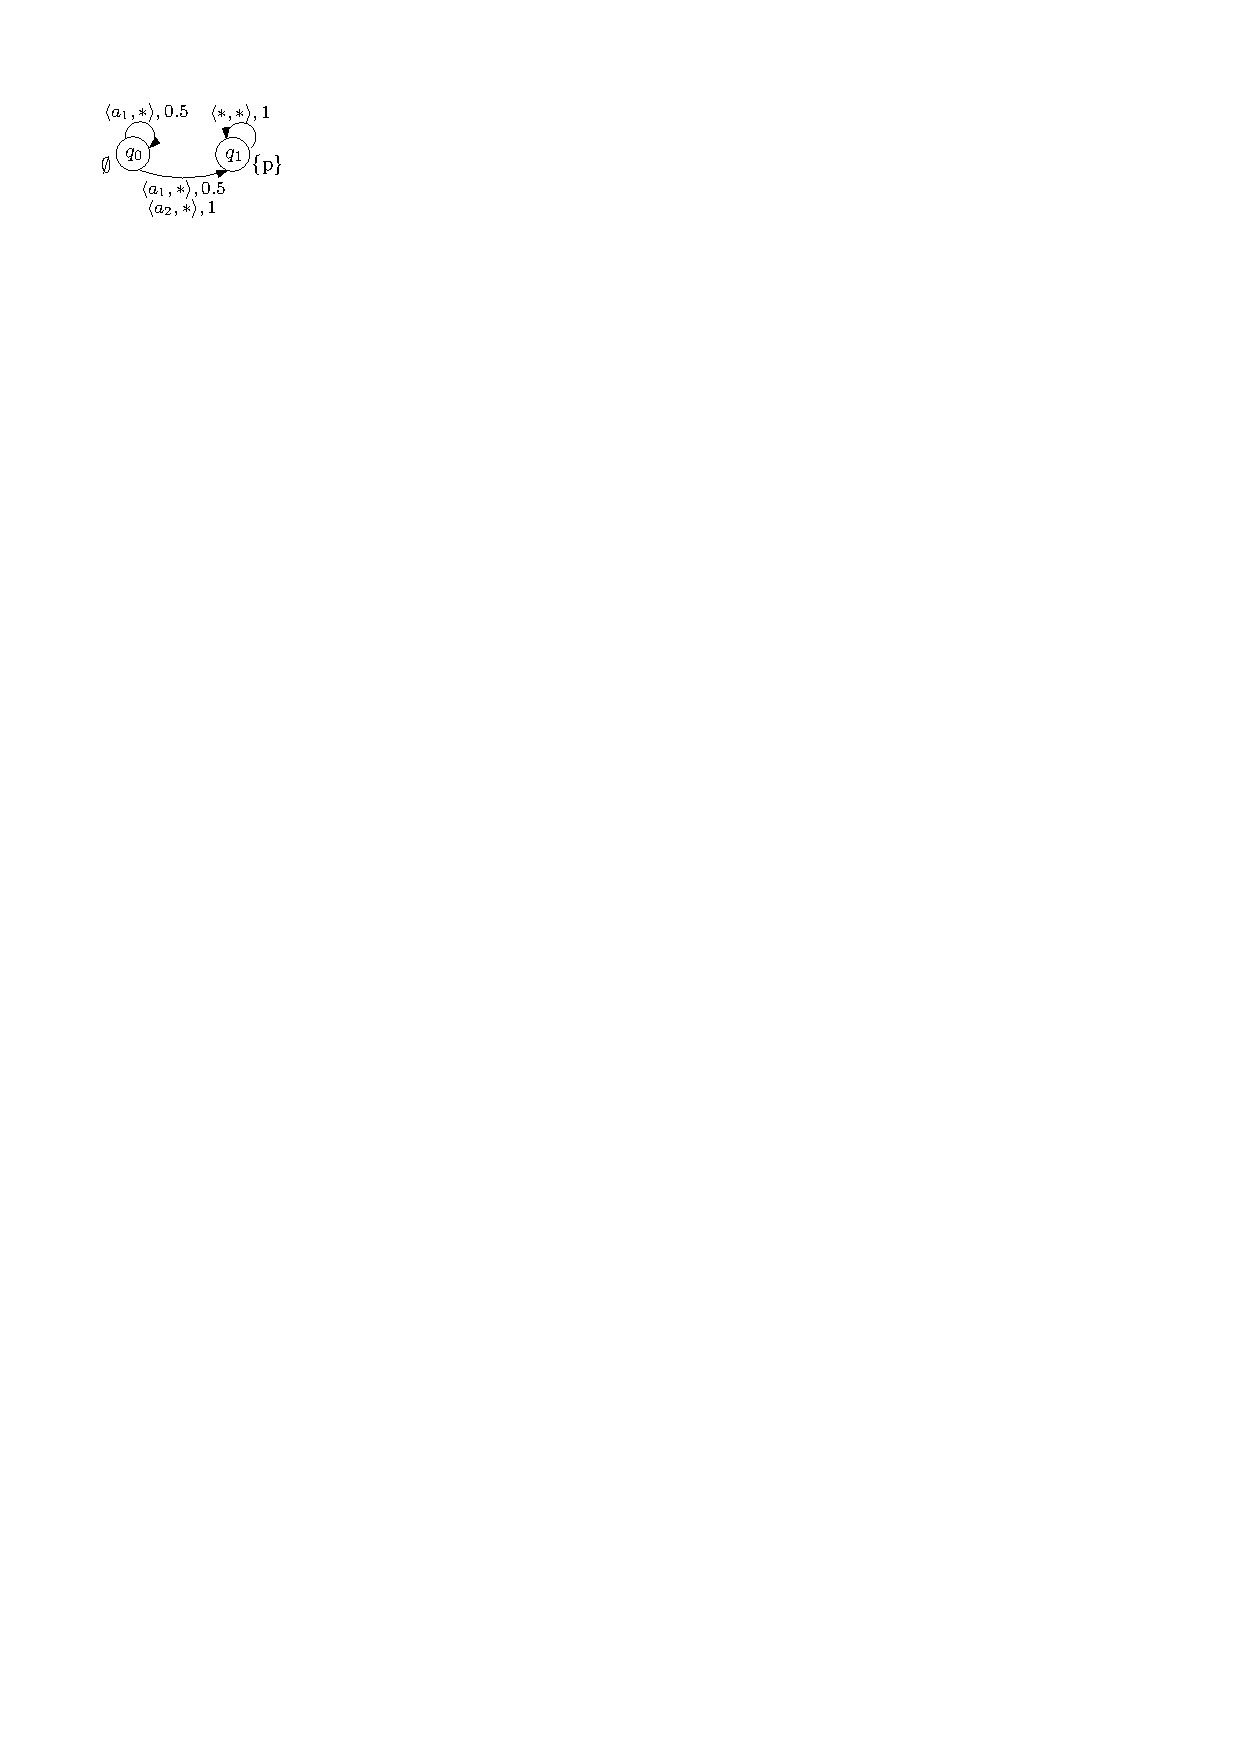
\includegraphics[width=0.18\textwidth]{figure//fig-example1}\\
  \caption{Example for memoryless property on \pamc, where $*\in\{a_1,a_2\}$.}\label{fig-example1}
\end{figure}

\begin{example}
Let us the pCGS $\calM=(\{1,2\},\{a_1,a_2\},\{q_0,q_1\}, \delta,\lambda, q_0)$ as shown in Figure \ref{fig-example1}, where for every $*\in\{a_1,a_2\}$,
\begin{itemize}
\item $\delta(q_0,\langle a_1,*\rangle, q_0)=0.5$ and $\delta(q_0,\langle a_1,*\rangle, q_1)=0.5$,
\item $\delta(q_0,\langle a_2,*\rangle, q_1)=1$,
\item $\delta(q_1,\dec,q_1)=1$ for every $\dec\in \{a_1,a_2\}^2$,
\item $\lambda(p)=\{q_1\}$.
\end{itemize}

Consider the closed \pamc state formula $\phi=\opA{\{1\}}^{\geq 0.5}\opX(\neg p \wedge \opX p)$ which states that
agent $1$ has a strategy such that whatever agent $2$ does, the probability to achieve the goal $\opX(\neg p \wedge \opX p)$
is no less than $0.5$. It is easy to see that there is no memoryless strategy for agent $1$ to achieve the goal, i.e.,
$\semantics{\phi}_\calM^r=\emptyset$. While $\semantics{\phi}_\calM^R=\{q_0\}$, as agent $1$ can use the strategy $\upsilon_{\{1\}}$
such that $\upsilon_{\{1\}}(q_0)(a_1)=1$ and $\upsilon_{\{1\}}(q_0q_0)(a_2)=1$.
\end{example}

\subsection{Randomized vs. Deterministic}
\begin{theorem}\label{thm-p2d}
Given a closed \pamc state formula $\phi$, let $\semantics{\phi}_\calM^p$ and $\semantics{\phi}_\calM^d$ respectively denote the set of states
satisfying $\phi$ under randomized and deterministic settings. Then,
$\semantics{\phi}_\calM^p=\semantics{\phi}_\calM^d$ under memoryful setting.
\end{theorem}
\begin{proof}
The proof is straightforward by induction on the structure of $\phi$.
We only need to consider principal formulae of the form $\opA{A}^{\sim c}\psi$ and $\opUA{A}^{\sim c}\psi$.
The proof for the case $\opA{A}^{\sim c}\psi$ follows from
Theorem \ref{thm-ltl2pa} and Lemma \ref{lemma-mc2spg}, while $\opUA{A}^{\sim c}\psi$
can be proved by switching players in the stochastic parity game.
\end{proof}

Let \pamc$^=$ be the logic by setting $\sim\in\{\geq,>,=\}$ in the \pamc.
Then, Theorem \ref{thm-p2d} will not hold for \pamc$^=$. We show this by the following example.




\begin{example}
Let us consider the pCGS
$\calM=(\{1,2\},\{a_1,a_2\},\{q_0,q_1\}, \delta,\lambda)$ as shown in Figure \ref{fig-example1} and the closed \pamc$^=$ state formula $\phi=\opA{\{1\}}\opX^{=0.75} p$.

In randomized setting, agent $1$ has a strategy $\upsilon_{\{1\}}$ such that for all strategies $\upsilon_{\{2\}}$ of agent $2$, $\Prb_{q_0}^{\upsilon_{\{1\}},\upsilon_{\{2\}}}(\{\rho\in \calP_{q_0}^{\upsilon_{\{1\}}, \upsilon_{\{2\}}}\mid \rho_1\in\semantics{p}_\calM^\xi\})=0.75$, where
$\upsilon_{\{1\}}(\pi)(a_1)=0.5$ and $\upsilon_{\{1\}}(\pi)(a_2)=0.5$. Therefore $q_0\in\semantics{p}_\calM^\xi$.
While, in deterministic setting, it is easy to see that $q_0\not\in\semantics{p}_\calM^\xi$.
\end{example}



\begin{figure}[h]
  \centering
  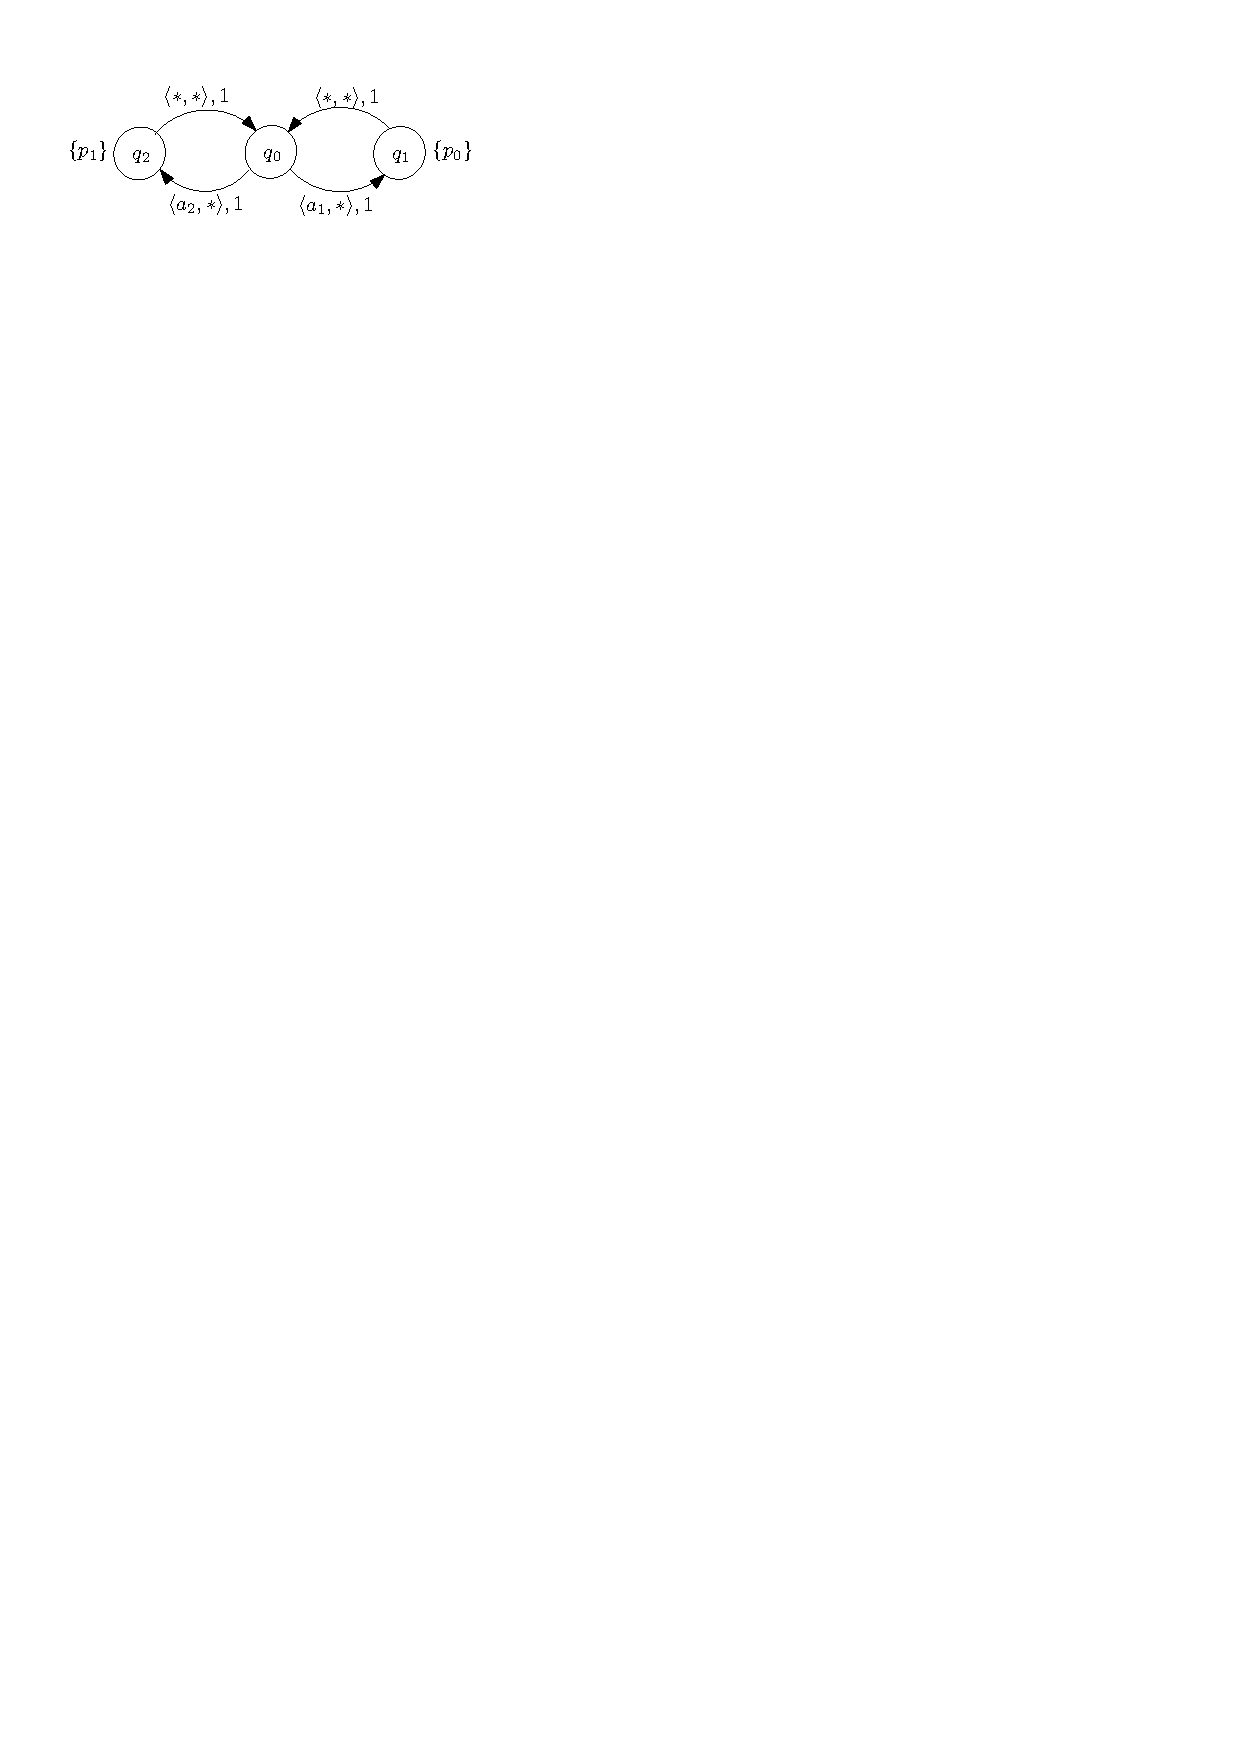
\includegraphics[width=0.35\textwidth]{figure//fig-example2}\\
  \caption{Example for determinacy, where $*\in\{a_1,a_2\}$.}\label{fig-example2}
\end{figure}


Under memoryless setting, \pamc does not have determinacy property as shown by the following example.
\begin{example}
Let us consider the pCGS
$\calM=(\{1,2\},\{a_1,a_2\},\{q_0,q_1,q_3\}, \delta,\lambda)$ as shown in Figure  \ref{fig-example2}
and the closed \pamc state formula $\phi=\opA{\{1\}}^{>0} (\mu_p Z. p_1 \wedge \mu_p Y. p_0)$.

Under randomized memoryless setting,  $q_0\in\semantics{\phi}_\calM^\xi$, while $q_0\not\in\semantics{\phi}_\calM^\xi$ under deterministic memoryless setting.
\end{example}
